\capitulo{5}{Aspectos relevantes del desarrollo del proyecto}

El desarrollo de este proyecto puede decirse que ha estado dividido principalmente en dos partes. La primera
fase estuvo relacionada con el diseño de la arquitectura, así como la elección del sistema gestor de bases de
datos. En la segunda fase, se diseñó todo lo relativo a la predicción de datos y a la elección de las
herramientas necesarias para dicha tarea.

\section{Diseño de la arquitectura y comparativa de los gestores de bases de datos}

Como ha sido mencionado en el párrafo anterior, en la primera fase se llevó a cabo el diseño de la
arquitectura del sistema, así como el desarrollo de los servicios que forman dicho sistema. Además,
se ha realizado una comparativa de diferentes sistemas gestores de bases de datos con el fin de elegir
el que mejor se adapte a nuestros requisitos.

Esta parte del desarrollo del proyecto ha sido publicada en la conferencia SOCO 2023 \cite{8364SOCO}. Esta publicación 
se incluye también en la sección F de los anexos.

\subsection{Diseño de la arquitectura}

La arquitectura del sistema estudiado se representa en la figura \ref{fig:Arquitectura}. El sistema
está formado por los siguientes sistemas software:
\begin{description}
    \item [AGV Coordinator] Es un servicio encargado de recibir la información enviada por los AGV a
        través de una conexión 5G/Wifi. Esta información está codificada como una cadena de bytes, que
        es decodificada y transformada a formato JSON. Estos mensajes son enviados al servicio 
        ``Receiver''. Este servicio ha sido desarrollado como parte de otro proyecto, por lo que no
        se detallará en este.
    \item [Simulator] Es, como su nombre en inglés indica, un servicio encargado de simular un AGV
        en caso de no disponer de AGV reales y sea necesario realizar pruebas.
    \item [Receiver] Este servicio recibe mensajes a través del protocolo UDP bien del ``AGV Coordinator''
        o bien del simulador, y se encarga de insertar dichos datos en la base de datos.
    \item [Database] Como su nombre indica, este servicio será la base de datos encargada de almacenar
        todos los datos recibidos.
\end{description}

\imagen{Arquitectura}{Diseño de la arquitectura}{1}

\subsection{Comparativa de Sistemas Gestores de Bases de Datos}

Inicialmente, se seleccionaron los cinco sistemas gestores de bases de datos para series temporales más populares 
según el ranking DB-Engines \cite{dbengines:rankingTSDBMS}:
\begin{enumerate}
    \item InfluxDB
    \item Prometheus
    \item Kdb+
    \item Graphite
    \item TimescaleDB
\end{enumerate}

A partir de esta lista de gestores, se ha realizado una comparación exhaustiva de los mismos según los requisitos 
del proyecto. Esta comparativa puede verse en el apartado B.5 de los anexos que se incluyen de forma complementaria 
a esta memoria.

Como resumen de dicha comparativa, tanto InfluxDB como TimescaleDB cumplen con los requisitos especificados. Finalmente,
el sistema escogido ha sido InfluxDB debido a su menor uso de recursos con un rendimiento suficiente y a 
la implementación por defecto de una herramienta de visualización de la información.

\subsection{Desarrollo de los servicios}

Una vez diseñada la arquitectura y el sistema gestor de bases de datos escogido, se procedió a desarrollar los
sistemas definidos. Todos estos sistemas se ejecutan cada uno en su contenedor de Docker independiente, los cuales 
se comunican entre sí a través de una red especificada en el archivo de configuración de docker compose.

\subsubsection{Simulator}
Inicialmente, no disponía de datos reales del AGV, por lo que la primera versión (Figura \ref{fig:v1sim}) simplemente generaba datos aleatorios
con campos aleatorios, y los enviaba al nodo ``Receiver'' por UDP utilizando el puerto 5004.

Después, se intentó desarrollar un simulador capaz de, valga la redundancia, simular el comportamiento de un AGV. Sin
embargo, una vez dispuse de datos reales del AGV, esta idea se descartó, pues simular dicha información de forma
precisa iba a ser demasiado complejo, y se escapa del objetivo de este proyecto. Por tanto, se decidió simular el
comportamiento del AGV leyendo los datos de un CSV (Figura \ref{fig:v2sim}) obtenido a partir de uno real.

\begin{figure}
    \centering
    \begin{subfigure}[b]{0.45\textwidth}
        \centering
        \includegraphics*[width=0.5\textwidth]{v1sim}
        \caption{Generación aleatoria}
        \label{fig:v1sim}
    \end{subfigure}
    \hfill
    \begin{subfigure}[b]{0.45\textwidth}
        \centering
        \includegraphics*[width=\textwidth]{v2sim}
        \caption{Generación por CSV}
        \label{fig:v2sim}
    \end{subfigure}
    \begin{subfigure}[b]{0.7\textwidth}
        \centering
        \includegraphics*[width=\textwidth]{sim}
        \caption{Versión final}
        \label{fig:sim}
    \end{subfigure}
    \caption{Diagramas de flujo del simulador}
    \label{fig:diagsim}
\end{figure}

Por último, en la versión final se unificaron los dos procedimientos, de forma que el comportamiento del simulador
se decide según lo especificado en un archivo de configuración.

\subsubsection{Receiver}

El funcionamiento del nodo ``Receiver'' es muy simple (Figura \ref{fig:recv}): escucha el puerto UDP 5004, y cuando recibe información, la inserta 
en la base de datos. Inicialmente, el servicio intentará conectarse a la base de datos. Si esta conexión falla un número
determinado de veces, el servicio fallará informando de que la conexión no ha podido realizarse.

\imagen{recv}{Diagrama de flujo del servicio ``Receiver''}{0.5}

\subsubsection{Database}

Este servicio simplemente inicia un contenedor de Docker con la base de datos. Es necesario sin embargo 
especificar las credenciales del usuario administrador que tendrá los permisos necesarios para insertar 
información en dicha base de datos.

\section{Modelo de predicción de datos}

La segunda fase se centró en el desarrollo y diseño del servicio de predicción de nuevos datos.
Se ha realizado un análisis comparativo de diferentes modelos predictivos, así como un análisis
de los datos recibidos por el AGV para hacer la mejor elección.

\subsection{Modificación de la arquitectura}

Ya que se ha pretendido desarrollar una arquitectura lo más modular posible, la predicción de la 
información se realiza desde un nuevo servicio. Por ende, la arquitectura modificada queda de la 
siguiente manera:

\imagen{Arquitectura2}{Arquitectura final}{1}

Este nuevo servicio se conecta directamente a la base de datos de la que extrae la 
información necesaria para hacer las predicciones. Una vez hechas se insertan en la base de datos 
para poder ser visualizadas en la utilidad web de la base de datos, Chronograf \cite{chronograf:docs}.

\subsection{Análisis de los datos}

Antes de hacer nada relativo a la predicción de los datos, necesitamos conocer que datos tenemos y cuáles 
queremos predecir. Del AGV recibimos los siguientes datos:
\begin{itemize}
    \item Tiempo: tiempo que ha pasado en segundos desde que se inicia el AGV.
    \item Encoder derecho: valor del codificador de la rueda derecha. Cuando el AGV avanza este valor se
        incrementa, y cuando retrocede se decrementa.
    \item Encoder izquierdo: igual al anterior, pero con la rueda izquierda.
    \item Corriente: dividido en límites inferior y superior.
    \item Medida batería: corriente medida en la batería.
    \item Error de guiado: distancia que el AGV está desviado de la banda magnética por la que se guía.
    \item Consigna de velocidad derecha: valor de la velocidad enviado a la rueda derecha.
    \item Consigna de velocidad izquierda: similar al anterior pero con la rueda izquierda.
    \item Display: valor recibido con información del AGV.
\end{itemize}

Cabe mencionar que, como los encoders derecho e izquierdo no nos muestran directamente la velocidad de las 
ruedas (Figura \ref{fig:datos_enc_derecho_sp}), antes hay que preprocesar dichos datos, restando cada valor con su anterior, obteniendo así el dato de la 
velocidad (Figura \ref{fig:datos_enc_derecho_dif}).

\begin{figure}[H]
    \centering
    \begin{subfigure}[b]{0.45\textwidth}
        \centering
        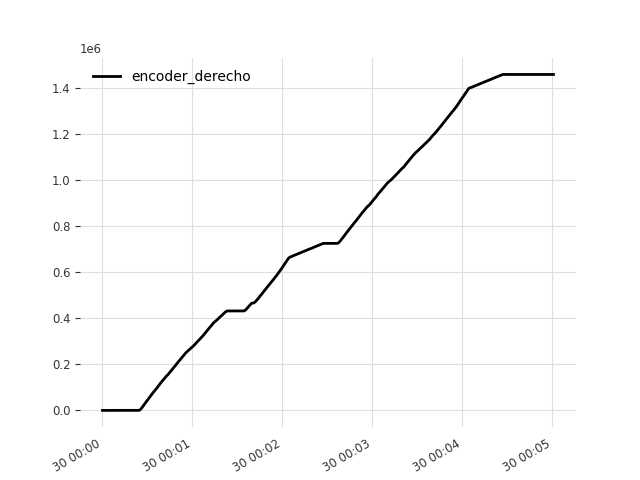
\includegraphics[width=\textwidth]{enc_derecho}
        \caption{Sin procesar}
        \label{fig:datos_enc_derecho_sp}
    \end{subfigure}
    \hfill
    \begin{subfigure}[b]{0.45\textwidth}
        \centering
        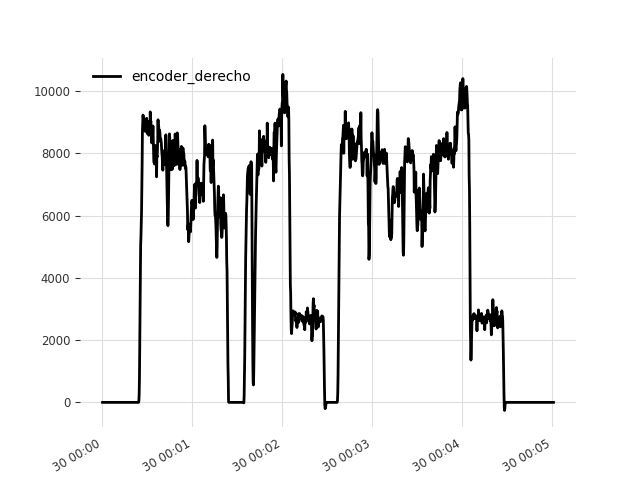
\includegraphics[width=\textwidth]{enc_derecho_dif}
        \caption{Después de diferenciación}
        \label{fig:datos_enc_derecho_dif}
    \end{subfigure}
    \caption{Datos del encoder derecho}
    \label{fig:datos_enc_derecho}
\end{figure}

El objetivo es realizar una predicción de los valores encoder derecho y encoder izquierdo para poder 
compararlos con los obtenidos y detectar posibles errores. Para ello, utilizamos valores anteriores de los 
mismos datos, así como los valores de las consignas de velocidad derecha e izquierda, pues su correlación 
es muy alta. Para predecir los valores derechos, y viceversa, se usan también los valores izquierdos, pues aunque su 
correlación no sea tan alta, también están correlacionados.
Ya que estos datos se mandan en intervalos de tiempo irregulares, el primer paso es agruparlos en ventanas de 200 milisegundos. 
Esto es así porque para realizar las predicciones es necesario que los datos de la serie temporal estén distribuidos 
de manera uniforme.

Las pruebas realizadas a los modelos han sido realizadas únicamente con el encoder derecho, pues al ser muy similar 
al encoder izquierdo se van a obtener resultados prácticamente idénticos en los dos casos, por lo que no merece 
la pena realizar las pruebas sobre los dos datos.

\subsection{Comparativa de modelos de predicción}

Al igual que con la comparativa de sistemas gestores de bases de datos, una comparativa exhaustiva de los modelos 
de predicción puede encontrarse en la sección B.6 de los anexos complementarios.

De dicha comparación se sacan las siguientes conclusiones:
\begin{itemize}
    \item El tiempo empleado para la optimización de los modelos no ha sido suficiente, pues los modelos
        supuestamente optimizados dan peores resultados, tanto en las métricas como en el tiempo de entrenamiento.
    \item El mejor modelo para predicciones a largo plazo es el Transformer por defecto, aunque N-HiTS da buenos
        resultados también con un tiempo de entrenamiento menor.
    \item Para predicciones a corto plazo, ARIMA resulta el mejor modelo.
\end{itemize}

Ya que nuestra intención es realizar predicciones a relativamente largo plazo, el modelo escogido ha sido el modelo 
Transformer. Podría haberse escogido también el modelo N-HiTS, pero como el modelo solo se entrena una vez el tiempo 
de entrenamiento tendrá una menor importancia comparada con el resto de métricas.

\subsection{Desarrollo del servicio}

Como se puede ver en la siguiente imagen (Figura \ref{fig:diagrama_forecast}), este servicio carga un modelo desde 
un archivo o bien lo entrena desde cero. Para poder entrenar dicho modelo, se necesita que la base de datos ya tenga 
datos cargados, por lo que la rutina de entrenamiento espera algunos minutos antes de empezar a entrenar para que 
haya los datos necesarios para poder realizar dicha tarea. La cantidad de tiempo a esperar antes de entrenar se especifica 
en un archivo de configuración.

En el caso de cargar el modelo desde un archivo, también es necesario esperar un tiempo a que la base de datos se cargue 
de información, pues es necesario escalar los datos antes de hacer la predicción. Dicha escala se ajusta según los datos 
introducidos, por lo que cuanto más tiempo esperamos en este paso, más parecida será a la especificada a la hora
de entrenar el modelo.

Los datos generados en la predicción son insertados a un ``bucket'' de la base de datos diferente al que están los datos.
Este ``bucket'' tiene un periodo de retención bajo. Esto significa que los datos insertados se eliminan después 
de cierto tiempo, pues no nos interesa guardar predicciones antiguas.

Existen dos versiones de este servicio: una utiliza una GPU de Nvidia para entrenar y la otra utiliza la CPU. Entrenar con
GPU es mucho más rápido que con CPU, por lo que siempre que se disponga de una es muy recomendable utilizar esta versión.
En caso de no disponer de una GPU, o de disponer de una que no soporte la versión 11.8 de CUDA, siempre puede utilizarse el 
servicio complementario.

\imagen{diagrama_forecast}{Diagrama del servicio de predicción.}{0.8}

\section{Despliegue del proyecto}

Cada servicio queda definido en un archivo ``Dockerfile'', que definirá el contenido y acciones de cada uno de los 
contenedores.

Todos estos servicios se inician utilizando la herramienta docker compose. Con esta herramienta podremos crear
una red virtual a la que se conectan los diferentes servicios para poder comunicarse entre sí, especificar los
puertos que usa cada contenedor, variables de entorno, volúmenes, etc. Con esta herramienta podemos también ver los registros de cada contenedor, lo que nos permitirá ver posibles errores 
y trazas de información.

Para interaccionar con la aplicación, se accede a una aplicación web contenida en el servicio ``Database'' llamada 
Chronograf \cite{chronograf:docs}. Esta aplicación se aloja en el puerto 8086, por lo que, suponiendo que el sistema 
se ejecuta de forma local, se accede a través de la url ``localhost:8086''. En caso de ejecutarse en un servidor remoto,
basta con cambiar ``localhost'' por la IP o nombre de dominio de dicho servidor.

\imagen{preds}{Plantilla con los gráficos con las predicciones}{1}

En la Figura \ref{fig:preds} podemos observar dicha utilidad, en la que se muestran las predicciones realizadas en 
naranja y los datos recibidos por el AGV en azul. Una explicación en detalle de como acceder y utilizar esta interfaz se da 
en la sección E.4 de los anexos.

\section{Mantenimiento del código}

Al final del desarrollo, se integraron en el proyecto las herramientas de integración continua Code Climate y 
Pylint. Gracias a estas herramientas, se localizaron y resolvieron errores estilísticos y de mantenibilidad del código.